\documentclass[8pt, A4]{article}

%Margenes de la pagina.  otra opcion, usar \usepackage{a4wide}
\usepackage[paper=a4paper, left=0.8cm, right=0.8cm, bottom=1.3cm, top=0.9cm]{geometry}
\usepackage{color}

%este paquete permite incluir acentos.  Notar que espera un formato ANSI-blah de archivo.  Si en lugar de eso se tiene un utf8 (usual en los linux), entonces usar \usepackage[utf8]{inputenc}
\usepackage[utf8]{inputenc}

%Este paquete es para que algunos titulos (como Tabla de Contenidos) esten en castellano
\usepackage[spanish]{babel}

%El siguiente paquete permite escribir la caratula facilmente
\usepackage{caratula}

\usepackage{aed2-symb,aed2-itef,aed2-tad,aed2-tokenizer,modulos_diseno, ./algorithms/clrscode3e}
\usepackage{framed}
\usepackage{amsmath}

\usepackage{graphicx}

%Datos para la caratula
\materia{Algoritmos y Estructuras de Datos III}

\titulo{Trabajo Pr\'actico 1 - Pato-lógico}


\integrante{Ortiz de Zarate, Juan Manuel}{403/10}{jmanuoz@gmail.com}
\integrante{Martelletti, Pablo}{849/11}{pmartelletti@gmail.com}
\integrante{Kujawski, Kevin}{459/10}{kevinkuja@gmail.com}
\integrante{Carreiro, Martin}{45/10}{carreiromartin@gmail.com}

\begin{document}
%numero de grupo
{\hfill\Huge 10} %
\includegraphics[width=2cm]{./patologico.png} \\ 
%esto construye la caractula
\maketitle 

 
 \tableofcontents

 \newpage

\section{Introducci\'on}
En el siguiente trabajo presentaremos la resolución a tres problemas que se nos dio a resolver. Mostraremos para cada uno
el algoritmo que utilizamos para resolverlo describiendo que técnicas de las vistas en clase utilizamos, mostraremos también
el análisis de complejidad de cada algoritmo y mostraremos gráficamente los resultados de las mediciones para ver si se cumple el análisis 
teórico.


  \newpage
\section{Problema 1}

\subsection{Enunciado}
El enunciado nos plantea una situación en donde tenemos un edificio con n pisos y personas en cada piso que quiere ir a planta baja. Para poder hacerlo, el edificio provee un 
ascensor que deberá buscar a las personas para poder bajarlas. 
Este ascensor posee energía y capacidad limitada que no le permite recorrer siempre todos los pisos y levantar todas las personas, por lo tanto queremos maximizar la cantidad
de personas a descender del edificio dado la cantidad de personas por piso, su energía y la capacidad.

\subsection{Soluci\'on}
La solución planteada utiliza Programación Dinámica a través de decisiones. Es decir, planteamos el problema de forma tal que en vez de maximizar la cantidad de personas que 
pueden descender, encontramos el máximo valor posible que va a estar ubicado entre cero y la cantidad de personas total en el edificio.\\
A continuación se explicará cómo se resolvió el problema:\\
Primero obtenemos la cantidad total de personas recorriendo el edificio dado, y buscaremos ese dicho máximo valor.
Para ello, utilizaremos la conocida búsqueda binaria en la cantidad de personas en el edificio, hasta encontrar el valor tal que el siguiente no sea posible levantarlo y sin embargo el número que estoy evaluando si.
Por lo tanto lo único que resta, es ver si se puede levantar esa cantidad de personas dada la capacidad del ascensor, su energía y un edificio. \\
Para poder levantar esas personas buscaremos el piso mínimo al que necesitamos ir para poder levantar la cantidad de personas requeridas$^*$. Recorreremos el edificio desde ese piso mínimo hacia abajo, en caso de
ser posible llegar hasta él y poder volver a descender, levantando la máxima cantidad de personas de cada piso en el camino hasta llenar la capacidad. Una vez completada, descenderemos a los pasajeros y volveremos a repetir el proceso
para el mismo piso en caso de que haya quedado gente, o el siguiente en caso de haberlo vaciado o no poder llegar por poca energía, hasta que levantemos la cantidad requerida (caso que devolveremos que se puede) o hasta que nos quedemos sin energía (caso que devolveremos que no se puede). Tener en cuenta que el piso elegido como mínimo puede contener más cantidad de gente que la requerida por lo tanto puede pasar que no levantemos gente y que sin embargo, descendamos la cantidad requeridad personas.\\
Para la demostración de la resolución, explicaremos por qué el piso elegido previamente es el correcto, y por qué la estrategia de levantar de arriba hacia abajo es verdadera.
Este piso mínimo es la mejor opción ya que si subimos más pisos estaríamos utilizando energía para levantar la misma cantidad de gente que podríamos encontrar en los pisos
inferiores, y no se puede ir más abajo porque si no, tenemos la cantidad de gente necesaria para poder levantar el valor pedido.\\
Definimos el mundo de las estrategias, como el conjunto de estrategias posibles y definimos estrategia como el método por el que se levanta gente. Cómo no nos interesa
la energía utilizada, ya que solo queremos ver si puede levantar la cantidad de personas mencionada, y no la optimalidad de energía, una estrategia estará conformada por el
conjunto de personas que levanta en cada piso. De este mundo de estrategias, tomaremos solo aquellas que su piso más alto en el cual levantan personas es el nuestro, y que
levanten la misma cantidad que nosotros. Este conjunto es distinto de vacío ya que es un conjunto acotado de personas y pisos, por lo tanto se van a poder levantar a partir de
cierta energía dada. Ahora queremos ver que nuestra estrategia se encuentra en este conjunto. Para ello, tomaremos una de esas estrategias E y veremos que se puede permutar de tal
forma que consigamos nuestra estrategia. Esta permutación se debe a que si la estrategia E 


\small {\textbf{*} Para ubicar este piso mínimo recorreremos el edificio desde abajo contando la cantida de personas en los pisos, hasta que el valor sea mayor o igual al requerido.}




\subsection{Pseudoc\'odigo}
\begin{codebox}
\Procname{$\proc{resolver}$ (\textbf{in} $capacidad$, \textbf{in} $energia$, \textbf{in} $pisos$)}{maximaCantidad}{Int}
\li		totalPersonas = SumaTotalPersonas(pisos);
\li		return BusquedaBinariaPersonas(0,totalPersonas, totalPersonas,energia,capacidad,pisos);
\end{codebox}

\begin{codebox}
\Procname{$\proc{SumaTotalPersonas}$ (\textbf{in} $pisos$)}{acum}{Int}
\li		\textbf{Para} cada piso p \Do
\li			acum = acum + genteEnPiso(p) \End
\end{codebox}

\begin{codebox}
\Procname{$\proc{BusquedaBinariaPersonas}$ (\textbf{in} $desde$, \textbf{in} $hasta$, \textbf{in} $total$,\textbf{in} $energia$, \textbf{in} $capacidad$, \textbf{in} $pisos$)}{acum}{Int}
\li		medio = (desde + hasta)/2;
\li		puedo = sePuedeLevantar(energia, capacidad, pisos, medio);
\li 		\textbf{Si} puedo \Do
\li				\textbf{Si} no se puede levantar el siguiente terminé
\li 				\textbf{Si no} busquedaBinariaPersonas en la siguiente mitad \End
\li 		\textbf{Si no} busquedaBinariaPersonas en la primera mitad
\end{codebox}

\begin{codebox}
\Procname{$\proc{sePuedeLevantar}$ (\textbf{in} $energia$, \textbf{in} $capacidad$, \textbf{in} $pisos$, \textbf{in} $personasABuscar$)}{sePuede}{Boolean}
\li 		\textbf{Para} cada piso empezando desde el piso minimo \Do
\li			\textbf{Si} tengoEnergiaParaLlegar y Hay Gente \Do
\li				\textbf{Si} el piso tiene mas gente que mi capacidad \Do
\li					sumoLoQueLevante
\li					veoSiPuedoVolverAEstePiso \End
\li				\textbf{Si no} \Do
\li					sumoLoQueLevante
\li					mientrasBajoSumoGenteParandoEnLosPisosQueHayGente \End \End
\li			\textbf{Si no} \Do
\li				AnotoLasQueNoLevanté \End \End
\li		return (cuantoLevante >= personasABuscar)
\end{codebox}


\subsection{Analisís de complejidad}	
Para averiguar cuanta gente hay en todo el edificio tenemos que recorrer todo el vector 'pisos' e ir sumando la cantidad de gente en cada piso. Eso nos cuesto O(n) donde n es la cantidad de pisos. Luego hacemos una búsqueda binaria sobre la cantidad total de gente que mediante la función sePuedeLevantar busca el máximo de gente que es posible cargar. La complejidad de la búsqueda binaria es de O(log cantGente) (esto es sabido, porque ya lo vimos en algoritmos y estructura de datos 2) y la complejidad de la función sePuedeLevantar en el peor caso (sería cuando tiene que irse hasta el último piso para poder levantar la cantidad de gente solicitada y tiene energía suficiente para levantarlos a todos) es de: \\
	O( $\sum\limits_{i=0}^{n} { ( \lceil (pisos[i]/capacidad) \rceil  + i}$ ) ) \\
Esto es porque por cada piso al que voy tengo que ir tantas veces tal que levante el total de gente de ese piso (eso es $\lceil$pisos[i]/capacidad$\rceil$) y luego en caso que me haya sobrado espacio voy recorriendo todos los pisos inferiores para llenar la capacidad restante.
Finalmente la complejidad total del ejercicio nos queda:\\
O( n + Log(g) * $\sum\limits_{i=0}^{n} { ( \lceil (pisos[i]/capacidad) \rceil  + i ) }$ ) \\
Donde n es la cantidad total de pisos y g la cantidad total de gente en todo el edificio.

\subsection{Tests y Gráficos}
Con respecto a los tests realizados, los mismos no se hicieron en cuanto a la complejidad (ya que al utilizar estructuras primitivas de java, podemos asegurar que la complejidad de cada una de sus operaciones es la que aparece en la documentación de ellas y por tanto, es la que detallamos en el apartado anterior), sino en cuanto a la cantidad de ciclos que realiza cada solución (más precisamente, la creación del árbol generador mínimo) para distintas instancias, de acuerdo a la cantidad de vértices (localidades) y aristas (enlaces) que posee cada una.
Como podemos apreciar en los siguientes gráficos, la cantidad de ciclos, para grafos en donde la cantidad de aristas es la misma, es directamente proporcional a la cantidad de vértices que contenga el mismo (figura 1). Es cierto que en algunos casos ésto no se cumple pero, en el caso promedio, a más cantidad de vértices, con igual cantidad de aristas, más ciclos tendrá que hacer nuestro algoritmo para encontrar el AGM válido. Los casos extremos serían aquellos en donde las aristas se insertan ordenados de la misma forma que los leerá nuestro algoritmo, donde la cantidad de ciclos se corresponde con la cantidad de vértices. Por el contrario, el peor caso se da cuando hay muchas aristas de 2 vértices que ya fueron visitados, de menor peso de aquellas que contengan 1 vértice visitado y otro sin visitar. De ésta forma, el algoritmo hará tantos ciclos como aristas tenga el vértice para, recién en la último, procesar el vértice y agregarlo al AGM.
\begin {center}
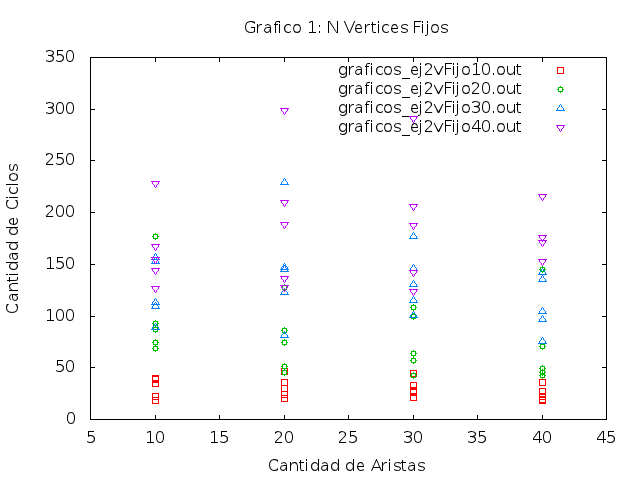
\includegraphics[width=8cm]{./graficos/grafico_vfijo.png}
% grafico.eps: 0x0 pixel, 300dpi, 0.00x0.00 cm, bb=50 50 410 302
\end {center} 
Por otro lado, y con respecto a la figura 2, donde la cantidad de aristas está fijo, vemos que la cantidad de ciclos que se llevan a cabo es netamente aleatorio, ya que, de acuerdo a cómo estén distribuidas las distintas aristas y sus pesos, es posible crear el AGM en n pasos, siendo n la cantida de vértices, o bien, en n x e(n), siendo e(n) la cantidad de aristas de n. El primer caso se daría sólo cuando el grafo que analizamos posee aristas minimas sin descubrir en todos los pasos, mientras que el peor caso, que sería el de recorrer todas las aristas del vértice, es el mismo que analizamos en el párrafo anterior.
\begin {center}
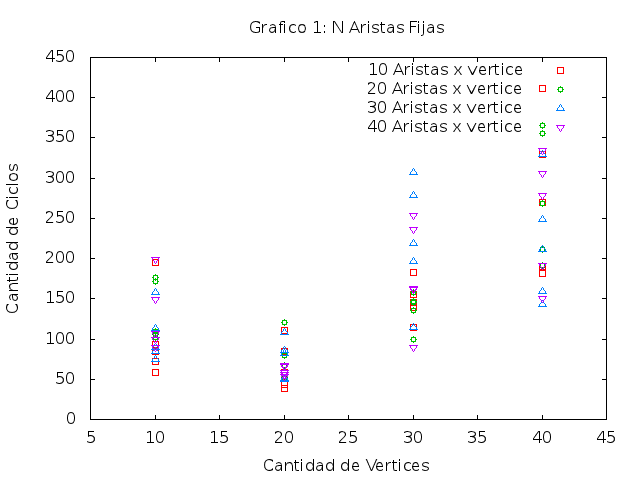
\includegraphics[width=8cm]{./graficos/grafico_efijo.png}
% grafico.eps: 0x0 pixel, 300dpi, 0.00x0.00 cm, bb=50 50 410 302
\end {center} 


\subsection{Conclusiones}
El problema nos mostró que podía ser encarado de distintas maneras dentro de la métodología de programación dinámica. Al principio habíamos utilizado una idea parecida a la de SubSetSum con memorization pero no podíamos hacer funcionar el algoritmo. Sin embargo, encaramos el problema a través de decisiones lo que nos ayudó a entender el principio de ptimalidad.

  \newpage
 \section{Problema 2}

\subsection{Enunciado}
En este ejercicio se nos solicita buscar el conjunto dominante mínimo y óptimo dado un grafo cualquiera. Este es un problema del tipo NP completo 
para el cual aún no se encontró forma de resolverlo polinomialmente pero tampoco se demostró que no sea posible solucionarlo con dicha complejidad.

\subsection{Soluci\'on}
Como todavía no se halló algoritmo alguno para resolverlo poliniomalmente y nosotros no somos investigadores/iluminados (aún) decidimos resolverlo
de manera exponencial. Para esto utilizamos el popular método (dicho en criollo) de quedarme con la mejor opción entre poner y no un nodo en el 
conjunto dominante. Este procedimiento lo que hace, básicamente, es analizar todas las soluciones posibles y agarrar la mejor de ellas. 
No nos pareció primordial agregarle memorization ya que su complejidad no mejoriría de forma considerable y tampoco nos pareció imperante 
preocuparnos por la complejidad de la función que chequea si el conjunto recibido es dominante, ya que, mientras sea polinimal, va ser despreciable 
al lado de la complejidad de analizar todas las soluciones (que como dijimos es exponencial).

\subsection{Pseudocódigo}

global grafoOriginal

\begin{codebox}
\Procname{$\proc{obtenerConjuntoDominanteMinimo}$ (\textbf{in} $Grafo$)}{mesetaMaxima}{Int}
\li	c = crearConj()
\li	grafoOriginal = Grafo
\li	return buscarMinimo(Grafo,c)
\end{codebox}

buscarMinimo(grafo, conjuntoDom){
	if(esDominante(conjuntoDom)){
		return conjuntoDom
	}else{
		vertice = grafo.obtenerVertice(); 
		grafo = grafo.sinUno()
		return min(buscarMinimo(grafo, conjuntoDom), buscarMinimo(grafo, conjuntoDom + vertice)
	}
}

esDominante(grafo, conjuntoDom){
	foreach(v en V(grafoOriginal)){
		if(conjuntoDom.esta?(v){
			continue
		}else{
			encontre = false
			foreach(ver en conjuntoDOm){
				if(ver.adyacentes.esta?(v))
					break
			}
			if(!encontre)
				return false
		}
	}
	return true
}

La complejidad de mi algoritmo es de 2^n * n³. Voy a demostrarlo por inducción:

Caso Base:

n = 1, si n tiene un solo nodo ver si es dominante me cuesta O(1) ya que recorrer los vertices del grafo original es una sola iteracion y no es posible recorrer sus aristas. Luego divido en el caso en el que uso a ese nodo en el conjunto dominante y el caso en que no. El caso en que no al no tener mas nodos con cual probar me va a devolver el grafo original y el otro caso también ya que el grafo original era el que contenía únicamente a ese nodo. Ambos casos ver si el conjunto es dominante cuesta O(1) ya que tiene a lo sumo una iteración para hacer. Por lo tanto el algoritmo costaría O(1) que es igual a O(2¹*1³).

Hipótesis inductiva:

Supongo que con n nodos la complejidad es 2^n * n³

Paso inductivo:

Quiero ver que con n+1 nodos la complejidad pertenece a 2^(n+1)*(n+1)³

Ver si el conjunto vacío es dominante me cuesta O(1) ya que en la primera iteración del grafoOriginal no es posible encontrar ningún vertice en el conjunto dominante o adyacente a él. Luego obtengo un nodo del grafo (grafo en el que me guarde todos los vertices, no el origianl) y busco el minimo conjunto dominante agregando ese nodo al conjunto o no, esto por hipótesis inductiva me cuesta 2 * (2^n * n³), ya que tengo que calcular 2 veces el conjunto minimo para n nodos. Por lo tanto la complejidad me termina costando  2^(n+1)*n³ y esto pertence a 2^(n+1)*(n+1)³. Con lo cual queda demostrada la complejidad.

Notar que esta complejidad esta por encima de la complejidad exacta, ya que el n³ variaría en cada iteración dependiendo de la cantidad de nodos en el conjuntoDominante.


\subsection{Peor Caso}

Como el algoritmo es exacto y recorre todas las soluciones posibles siempre obtiene la mejor de ellas. Por lo tanto no existe una 'peor' instancia
en la que la solución devuelta sea sub-óptima, siempre devuelve la mejor.

\subsection{Tests y análisis}




  \newpage
\section{Algoritmo Goloso}

\subsection{Soluci\'on}

Proponemos una solución heuristica golosa para encontrar un conjunto dominante de un grafo lo mas pequeño posible con una complejidad polinomial.\\
Para ello nos basamos en una estrategia de selección de nodos dominantes, la cual consiste en elegir el nodo que mas adyacentes no cubiertas tenga (es decir, que todavía no fueron dominadas) y verificando en cada iteración si el conjunto actual es dominante. En base a diferentes estrategias y tipos de grafos (estrella, bipartitos, completos, estrellas unidas, caminos, ciclos) que fuimos observando, elegimos esta ya que fue la que más nos convenció y mejores resultados nos dió debido a que siempre intenta seleccionar el nodo que mas pueda dominar a otros nodos reduciendo el conjunto de los no cubiertos y acercandose a una mejor solución del problema. 

\subsection{Pseudocódigo}

\begin{codebox}
\Procname{$\proc{MCDGreedy}$ (\textbf{in} $Grafo$)}{conjuntoDomGoloso}{ConjDeVértices}
\li	vértices = lista de vértices del grafo	\RComment O(n)
\li	dominantes = conjunto vacio de vértices	
\li	\textbf{Mientras} no estén TodasCubiertas(vértices) \Do \RComment O($n^3$)
\li 		Ordeno los vértices por la cantidad adyacentes que tenga no cubiertas (sin dominar), de mayor a menor. \RComment O(n*log(n))
\li 		Elijo como dominante al primero de la lista y lo agrego al conjunto de \textbf{dominantes} \RComment O(n)
\li 		Saco de la lista de vértices al elegido \RComment O(n)
\li 		ActualizarGradoSinDominar(elegido) \RComment Actualizo los nodos del grafo,\\ disminuyendo la cantidad de \textit{grado sin dominar} de los adyacentes al elegido, y de los adyacentes a estos.  O($n^2$)
\End
\li	\textbf{return} dominantes
\end{codebox}

\begin{codebox}
\Procname{$\proc{TodasCubiertas}$ (\textbf{in} $ListaDeVertices$)}{result}{Boolean}
\li 	\textbf{Mientras} haya vértices en la lista \Do
\li 		\textbf{Si} el vértice no esta dominado \Do
\li 			\textbf{return} falso \End \End
\li 	\textbf{return} verdadero
\end{codebox}

\begin{codebox}
\Procname{$\proc{ActualizarGradoSinDominar}$ (\textbf{in} $Vertice elegido$)}{}{}
\li 	Marcar al vértice elegido como dominado.
\li 	unionDeAdyacentes = lista de vértices vacia, que luego se usará para actualizar.
\li 	\textbf{Mientras} haya vértices en la lista de adyacentes al \textbf{elegido} \Do
\li 		\textbf{Si} el vértice \textit{elegido} no estaba dominado \Do
\li 			Decremento en uno el grado de adyacentes sin dominar del nodo actual \End
\li 		\textbf{Si} el nodo actual \textit{elegido} no estaba dominado \Do
\li 			Agrego los nodos adyacentes a la lista \textit{unionDeAdyacentes} \End
\li 		Marco al nodo actual como dominado. \End
\li 	\textbf{Mientras} haya vértices en la lista unionDeAdyacentes \Do 
\li 			Decremento en uno el grado de adyacentes sin dominar del nodo actual \End %\RComment Recorro unionDeAdyacentes para actualizar\\  el grado de nodos adyacentes sin dominar
\end{codebox}

\section{Análisis de Complejidad}

La complejidad del algoritmo es de O($n^3$)

El algoritmo comienza creando una lista de vértices en O(n).\\
Luego entra en un ciclo que como máximo será lineal en la cantidad de vértices. En cada iteración deberá comprobar si el conjunto actual de vértices elegidos domina todo el grafo O($n^2$), ordenar todos los vértices O(n*log(n)), elegir un vértice O(1), removerlo de la lista O(n) y finalmente actualizar el atributo de los grados sin dominar adyacentes de cada nodo O($n^2$), esto es porque para los adyacentes del nodo elegido y a su vez para los adyacentes de estos tengo que bajar en uno este atributo, recorrer los adyacentes me lleva O(n) y por cada adyacente recorrer sus adyacentes también me lleva O(n), O(n) * O(n) = O($n^2$).\\

Por lo tanto, la complejidad nos queda:\\
O(n) + O(n) * (O($n^2$) + O(n*log(n) + O(n) + O($n^2$)) = O($n^3$)\\\\

La complejidad final del algoritmo goloso es de O($n^3$), cumpliendo el objetivo de ser polinomial.


\subsection{Peor Caso}

Al ser una heurística, en cierto casos la solución no es la optima que podría dar un algoritmo exacto, pero aún asi es correcta.
Los peores casos, donde se produce una diferencia en el tamaño de conjunto dominante respecto a la optima, se suelen dar en grafos en los que varios nodos tienen el mismo grado o hay pequeña diferencia, y esto es debido que para la elección del vertice dominante en cada iteración nos quedamos con el que mayor grado de nodos adyacentes no cubiertos tenga y si hay varios con esta misma característica puede pasar que el nodo seleccionado no sea conveniente a futuro para llegar a una solución optima.

En los siguientes ejemplos de grafos se puede apreciar mejor:

\begin {center}
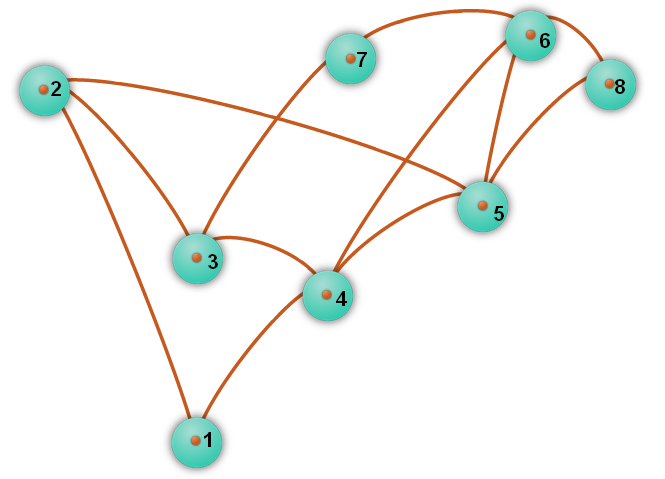
\includegraphics[width=8cm]{./graficos/grafo.png}
% grafico.eps: 0x0 pixel, 300dpi, 0.00x0.00 cm, bb=50 50 410 302
\end {center} 
La solución optima proporcionada por el algoritmo exacto es {6,2}, mientras que el goloso devuelve {4,3,5}, ya que como los nodos 6,4 y 5 tienen el mismo grado, al momento de la elección se decide por el 4 provocando esta diferencia en el tamaño del conjunto con respecto a la solución optima.

\begin {center}
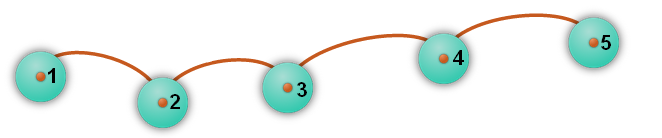
\includegraphics[width=8cm]{./graficos/grafo_camino.png}
% grafico.eps: 0x0 pixel, 300dpi, 0.00x0.00 cm, bb=50 50 410 302
\end {center} 
La solución óptima proporcionada por el algoritmo exacto es {2,4}, mientras que el goloso podría devolver {3,2,5}, ya que como los nodos 2, 3 y 4 tienen el mismo grado, si se decide por el 3, dejaría a todos los demas nodos con 1 grado sin dominar y faltando los dos extremos, provocando que si o si se necesite cubrirlos o elegirlos como dominantes, haciendo que el conjunto tenga tamaño 3 y no 2 como el exacto.

\subsection{Tests y análisis}

En los gráficos que aparece a continuación  se puede notar que a medida que la cantidad de nodos aumenta, el algoritmo dibuja un comportamiento que se asemeja a O($n^3$) en relación a la cantidad de ciclos y el tiempo en nanosegundos.\\

\begin {center}
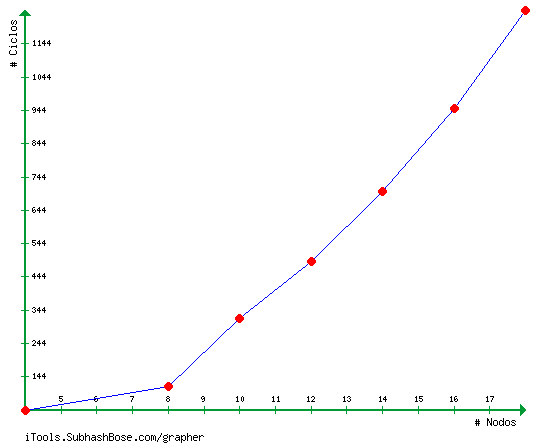
\includegraphics[width=8cm]{./graficos/goloso_1.png}
% grafico.eps: 0x0 pixel, 300dpi, 0.00x0.00 cm, bb=50 50 410 302
\end {center} 

\begin {center}
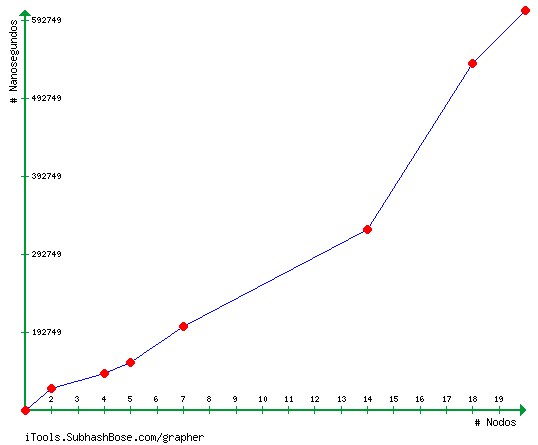
\includegraphics[width=8cm]{./graficos/goloso_2.png}
% grafico.eps: 0x0 pixel, 300dpi, 0.00x0.00 cm, bb=50 50 410 302
\end {center}

  \newpage
%\section{Apéndice}

$^{1}$http://docs.oracle.com/javase/6/docs/api/java/util/ArrayList.html

%  \newpage

\end{document}
